\section{项目流程设计}
\subsection{调研部分}
\begin{enumerate}
    \item 在设计治未病知信行问卷前,对20名社区居民进行访谈,目的在于了解居民健康需求、社区健康宣传和实际服务,居民获知信息渠道、居民关注的养生话题和日常养生行为。
    \item 设计相应知识、信念、行为三维度的题目,并交予相关专家评议通过。
    \item 发放问卷,回收分析,撰写统计报告。
\end{enumerate}
\subsection{干预部分}
\begin{enumerate}
    \item 建立微信公众号,确定受众、选题范围和相关传播策略。
    \item 招募写作成员并进行试写,之后进行正常推送,并且尽量推广到其他平台。
    \item 搜集用户对于平台信息的反馈,通过IP追踪等方法研究受干预群体的知信行情况。
\end{enumerate}
\begin{figure}[th]
	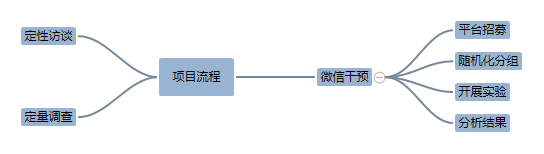
\includegraphics[width=\textwidth]{newprocess.png}
	\centering
	\caption{项目设计简图}
\end{figure}